\begin{figure}[p]\centering
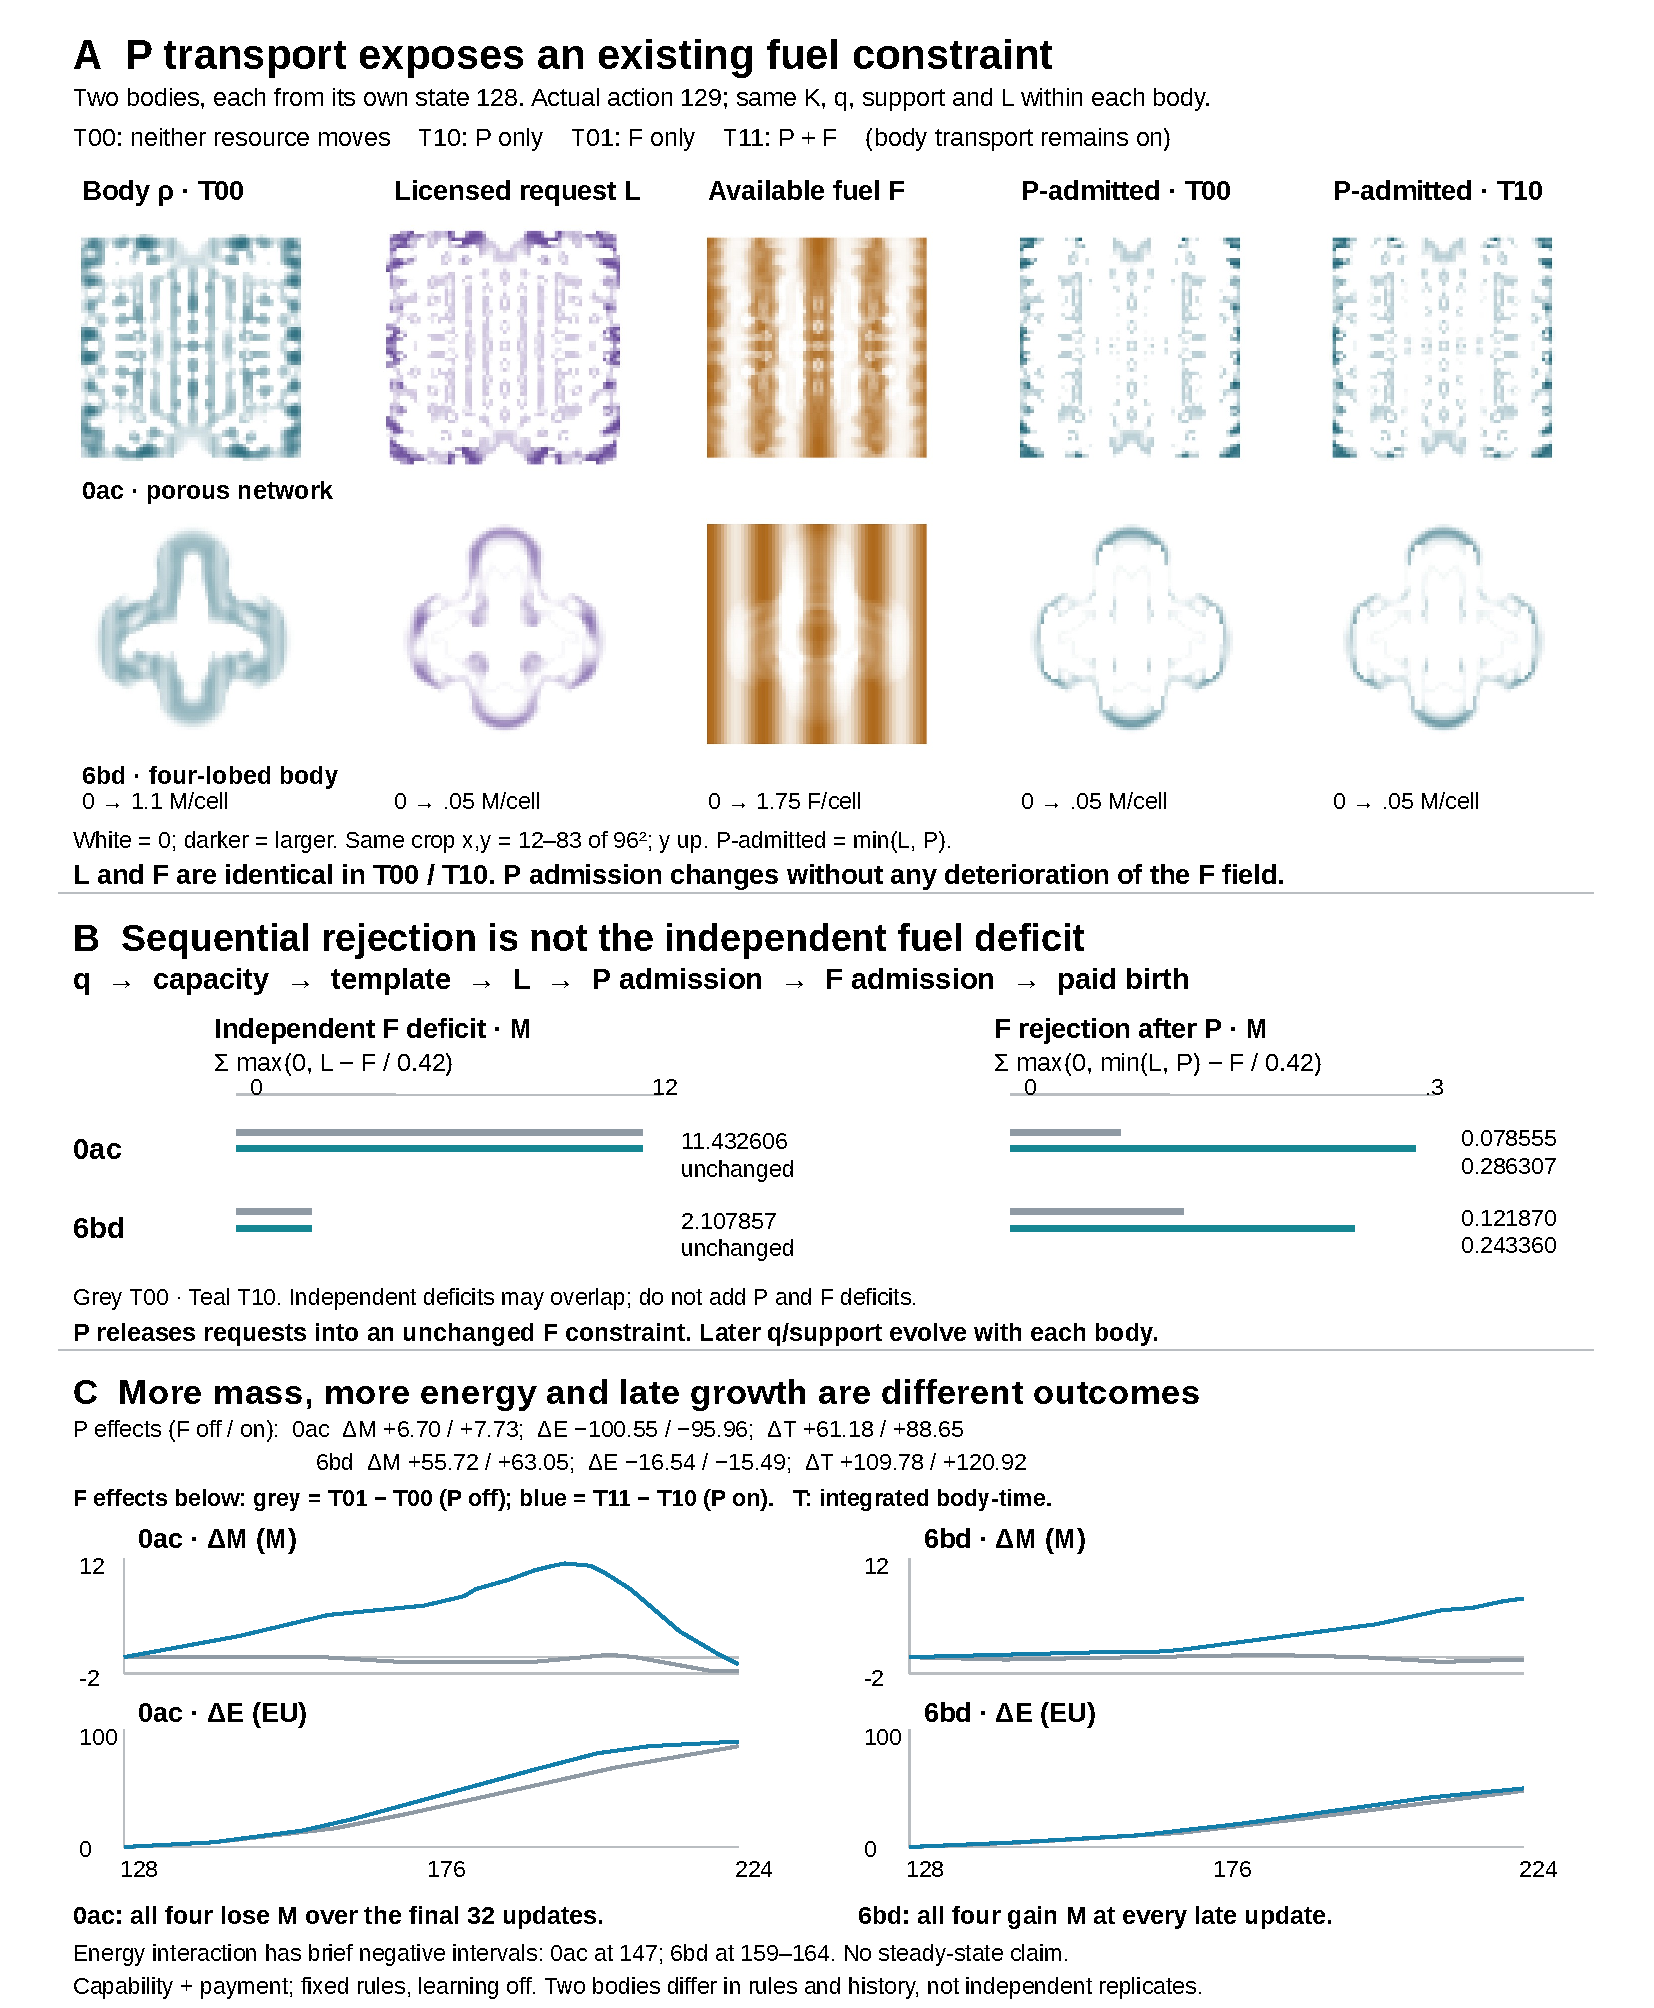
\includegraphics[width=\linewidth,height=.75\textheight,keepaspectratio]{figures/main/resource_constraints/resource_constraint_unmasking.pdf}
\caption{\textbf{P transport exposes fuel constraints without worsening fuel supply.}
\textbf{A,} Actual action 129 fields in two bodies continued from their own state 128. Fixed original-coordinate windows show T00 reference density, common licensed request $L$, common available fuel, and P-admitted requests with P transport off/on (T00/T10). Within each body, $K$, $q$, template support and $L$ match; F is identical pointwise.
\textbf{B,} The sequential capacity--template--P--F rule exposes more F rejection when P admits more requests, although the independent F deficit is unchanged. The quantities use separate scales; overlapping P/F deficits must not be added.
\textbf{C,} P increases final mass and body-time while reducing energy. Full-window F effects increase energy but change mass differently across bodies and time. All four 0ac branches lose mass over their final 32 updates; all four 6bd branches grow at every late update. Energy interaction is briefly negative despite positive endpoints. Capabilities and their actual payment change together; rules are fixed and learning is off. This is a conditional resource comparison, not an experience-adaptation test.}
\label{fig:allocation-feedback}\end{figure}
